\documentclass[a4paper,10pt]{article}

\usepackage[headheight=0pt,headsep=0pt,footskip=3.5cm]{geometry}

\usepackage{epsfig}
\renewcommand{\figurename}{Figura}
\usepackage{float}

\usepackage{tocloft}
\renewcommand{\cftsecleader}{\cftdotfill{\cftdotsep}}
\renewcommand{\contentsname}{Contenidos}

\usepackage{amssymb}

\begin{document}
\tableofcontents

\pagebreak

\section{Introducción}
En el presente informe se describen las tareas, realizadas en el laboratorio
GrIDComD, que fueron llevadas a cabo durante la ejecución de la Práctica Profesional
Supervisada correspondiente a la carreara Ingeniería en Computación por parte del autor de
este documento. El objetivo de la práctica fue diseñar e implementar un simulador de bajo costo
de las señales recibidas en vuelo por los satélites pertenecientes al sistema DCS.

\section{Lugar de trabajo}
\subsection{Descripción de la entidad}
\subsection{Organigrama}

\section{Sistema DCS}

La principal tecnología que el autor necesitó incorporar para la realización de la práctica, fue el conocimiento
sobre el Sistema Satelital Argentino de Recolección de Datos Ambientales (DCS). 
\par
Implementado por la comisión Nacional de Actividades Espaciales(CONAE), dicho sistema tiene como objetivo el
recolectar datos ambientales de distintos puntos del planeta, principalmente lugares inhóspitos y de difícil acceso. Este está formado
por tres segmentos:

\begin{itemize}
\item Segmento espacial: conformado por todos los elementos del sistema que se encuentran a bordo de satélites, este tiene como finalidad
recibir y almacenar los datos registrados, además de dar la posibilidad de obtenerlos desde la tierra, no sin antes preprocesarlos.
\item Plataformas: hace referencia a las plataformas que tienen como tarea recolectar datos de su entorno y transmitirlos a los satélites (DCP).
\item Segmento terrestre: compuesto por las facilidades que permiten descargar las lecturas almacenadas en los satélites y su disposición
a los usuarios para su análisis mediante servidores en línea o bien otros tipos de soportes de distribución de datos.
\end{itemize}
De este modo, los datos son leídos por las plataformas, quienes los transmiten a los satélites, donde son preprocesados para luego ser descargados 
y puesto a disposición de los usuarios mediante estaciones terrenas.


\subsection{Características de las señales}
Las señales transmitidas por las DCP poseen las siguientes características:
\begin{itemize}
\item Frecuencia de portadora de 401.55Mhz. Cabe destacar que si bien la posibilidad de colisión entre mensajes puede llevar a la pérdida de estos, 
los corrimientos de Doppler según la ubicación de cada DCP puede ayudar a separar estos en frecuencia.
\item Utiliza modulación PSK binaria con un $\theta$ de $\pm $ 1.1 rad $ \approx 63^o$.
\item Tasa de bits de 400bps.
\item Codificación Manchester.
\item Intervalo entre transmisiones de entre 30 y 220 segundos.
\end{itemize}

\subsection{Formato del mensaje}
El formato del mensaje enviado por las DCP se puede apreciar en la figura ~\ref{formatoMensaje}

\begin{figure}[H]
\centering
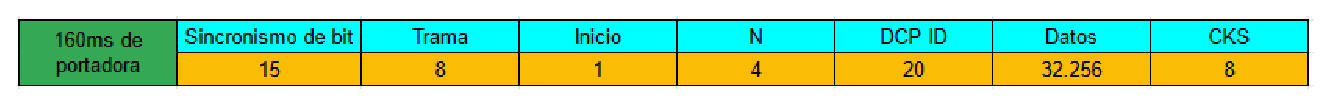
\epsfig{file=FigFormato.eps, width=14.0cm, height=1.1cm}
\caption{Formato del mensaje transmitido}
\label{formatoMensaje}
\end{figure}

Como se muestra, en primer lugar se transmite únicamente la señal portadora durante 160ms, con el fin de que el receptor detecte la señal y se sincronice con esta. Luego, se envía el mensaje en si, el cual consta de los siguientes campos:
\begin{itemize}
\item Sincronismo de bit: consta de 15 unos.
\item Trama: 8 bits que sirven para indicar al receptor que se está recibiendo un mensaje del sistema y solucionar la ambigüedad de $\pi$ en la fase.
\item Bit inicial: un uno que marcará el inicio de los bits a relevantes al mensaje a partir del primero luego de este.
\item N: campo de 4 bits que indica el tamaño en paquetes de 32 bits del campo de datos. Puede tomar valores entre 1 y 8, por esto el campo de datos puede tener entre 32 y 256 bits de largo.
\item DCP ID: 20 bits cuya función es identificar la plataforma que envía el mensaje.
\item Datos: los datos propiamente dichos.
\item CKS: checksum de 8 bits formada a partir de realizar el XOR entre todos los bytes que componen al resto de campos del mensaje. Este sirve para detectar errores en los bits recibidos.
\end{itemize}

\section{Implementación del simulador}
\section{Experiencia}
\section{Conclusiones}
\end{document}